
\documentclass[tikz,border=1pt]{standalone}

\usepackage{bm}

\usetikzlibrary{decorations.markings,arrows.meta}

% 電気力線のスタイル設定
\tikzset{eflineA/.style={thick,postaction=
    {decorate,decoration={
    markings, mark=at position 0.339 with {\arrow{Stealth}}}
    }}}
\tikzset{eflineB/.style={thick,postaction=
    {decorate,decoration={
    markings, mark=at position 0.488 with {\arrow{Stealth}}}
    }}}
\tikzset{eflineC/.style={thick,postaction=
    {decorate,decoration={
    markings, mark=at position 0.588 with {\arrow{Stealth}}}
    }}}
\tikzset{eflineD/.style={thick,postaction=
    {decorate,decoration={
    markings, mark=at position 0.577 with {\arrow{Stealth}}}
    }}}
\tikzset{eflineE/.style={thick,postaction=
    {decorate,decoration={
    markings, mark=at position 0.472 with {\arrow{Stealth}}}
    }}}
\tikzset{eflineF/.style={thick,postaction=
    {decorate,decoration={
    markings, mark=at position 0.642 with {\arrow{Stealth}}}
    }}}
\tikzset{eflineG/.style={thick,postaction=
    {decorate,decoration={
    markings, mark=at position 0.735 with {\arrow{Stealth}}}
    }}}

\begin{document}

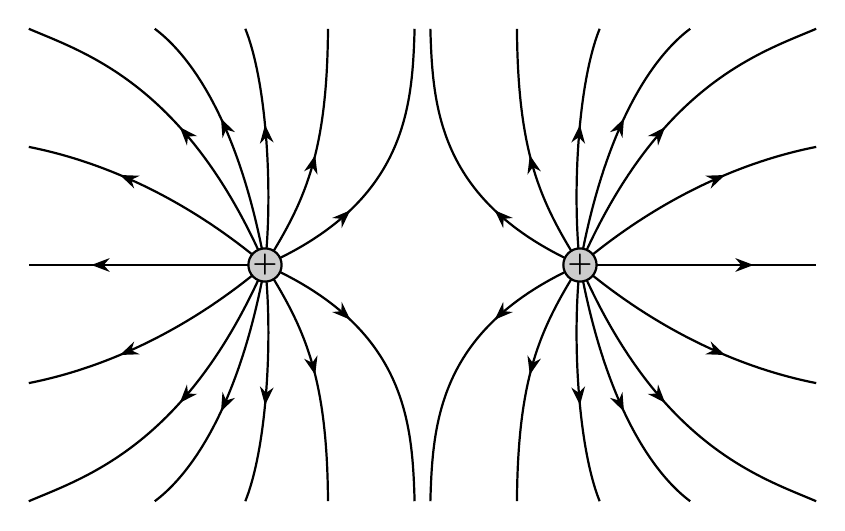
\begin{tikzpicture}

\pgfmathsetmacro{\xmax}{5}
\pgfmathsetmacro{\ymax}{3}

\pgfmathsetmacro{\X}{2}

\pgfmathsetmacro{\xa}{.1}
\pgfmathsetmacro{\ya}{3}
\pgfmathsetmacro{\xb}{.13}
\pgfmathsetmacro{\yb}{2}
\pgfmathsetmacro{\xc}{.2}
\pgfmathsetmacro{\yc}{.8}

\pgfmathsetmacro{\xd}{1.2}
\pgfmathsetmacro{\yd}{3}
\pgfmathsetmacro{\xe}{1.21}
\pgfmathsetmacro{\ye}{1.4}
\pgfmathsetmacro{\xf}{1.5}
\pgfmathsetmacro{\yf}{.8}

\pgfmathsetmacro{\xg}{2.25}
\pgfmathsetmacro{\yg}{3}
\pgfmathsetmacro{\xh}{1.97}
\pgfmathsetmacro{\yh}{2.3}
\pgfmathsetmacro{\xi}{1.9}
\pgfmathsetmacro{\yi}{.9}

\pgfmathsetmacro{\xj}{3.4}
\pgfmathsetmacro{\yj}{3}
\pgfmathsetmacro{\xk}{3.2}
\pgfmathsetmacro{\yk}{2.85}
\pgfmathsetmacro{\xl}{2.4}
\pgfmathsetmacro{\yl}{2.2}

\pgfmathsetmacro{\xm}{5}
\pgfmathsetmacro{\ym}{3}
\pgfmathsetmacro{\xn}{4.3}
\pgfmathsetmacro{\yn}{2.7}
\pgfmathsetmacro{\xo}{3}
\pgfmathsetmacro{\yo}{2.3}

\pgfmathsetmacro{\xp}{5}
\pgfmathsetmacro{\yp}{1.5}
\pgfmathsetmacro{\xq}{4.5}
\pgfmathsetmacro{\yq}{1.4}
\pgfmathsetmacro{\xr}{3.3}
\pgfmathsetmacro{\yr}{1.1}

% 補助方眼
%  \draw[step=1,thin,dotted] (-\xmax,-\ymax) grid (\xmax,\ymax);
%  \draw[->] (-\xmax,0) -- (\xmax,0) node[right] {x};
%  \draw[->] (0,-\ymax) -- (0,\ymax) node[above] {y};

% 補助楕円
%   \draw (-\X-0.5,0) circle [x radius=17mm, y radius=18.5mm];
%   \draw (\X+0.5,0) circle [x radius=17mm, y radius=18.5mm];

%　第2象限
\draw[eflineA]
    (-\X,0)..controls(-\xc,\yc) and (-\xb,\yb)..(-\xa,\ya);
\draw[eflineB]
    (-\X,0)..controls(-\xf,\yf) and (-\xe,\ye)..(-\xd,\yd);
\draw[eflineC]
    (-\X,0)..controls(-\xi,\yi) and (-\xh,\yh)..(-\xg,\yg);
\draw[eflineD]
    (-\X,0)..controls(-\xl,\yl) and (-\xk,\yk)..(-\xj,\yj);
\draw[eflineE]
    (-\X,0)..controls(-\xo,\yo) and (-\xn,\yn)..(-\xm,\ym);
\draw[eflineF]
    (-\X,0)..controls(-\xr,\yr) and (-\xq,\yq)..(-\xp,\yp);

% 第3象限
\draw[eflineA]
    (-\X,0)..controls(-\xc,-\yc) and (-\xb,-\yb)..(-\xa,-\ya);
\draw[eflineB]
    (-\X,0)..controls(-\xf,-\yf) and (-\xe,-\ye)..(-\xd,-\yd);
\draw[eflineC]
    (-\X,0)..controls(-\xi,-\yi) and (-\xh,-\yh)..(-\xg,-\yg);
\draw[eflineD]
    (-\X,0)..controls(-\xl,-\yl) and (-\xk,-\yk)..(-\xj,-\yj);
\draw[eflineE]
    (-\X,0)..controls(-\xo,-\yo) and (-\xn,-\yn)..(-\xm,-\ym);
\draw[eflineF]
    (-\X,0)..controls(-\xr,-\yr) and (-\xq,-\yq)..(-\xp,-\yp);

% 第1象限
\draw[eflineA]
    (\X,0)..controls(\xc,\yc) and (\xb,\yb)..(\xa,\ya);
\draw[eflineB]
    (\X,0)..controls(\xf,\yf) and (\xe,\ye)..(\xd,\yd);
\draw[eflineC]
    (\X,0)..controls(\xi,\yi) and (\xh,\yh)..(\xg,\yg);
\draw[eflineD]
    (\X,0)..controls(\xl,\yl) and (\xk,\yk)..(\xj,\yj);
\draw[eflineE]
    (\X,0)..controls(\xo,\yo) and (\xn,\yn)..(\xm,\ym);
\draw[eflineF]
    (\X,0)..controls(\xr,\yr) and (\xq,\yq)..(\xp,\yp);

% 第4象限
\draw[eflineA]
    (\X,0)..controls(\xc,-\yc) and (\xb,-\yb)..(\xa,-\ya);
\draw[eflineB]
    (\X,0)..controls(\xf,-\yf) and (\xe,-\ye)..(\xd,-\yd);
\draw[eflineC]
    (\X,0)..controls(\xi,-\yi) and (\xh,-\yh)..(\xg,-\yg);
\draw[eflineD]
    (\X,0)..controls(\xl,-\yl) and (\xk,-\yk)..(\xj,-\yj);
\draw[eflineE]
    (\X,0)..controls(\xo,-\yo) and (\xn,-\yn)..(\xm,-\ym);
\draw[eflineF]
    (\X,0)..controls(\xr,-\yr) and (\xq,-\yq)..(\xp,-\yp);

% x軸上の等電位線
\draw[eflineG] (\X,0) -- (\xmax,0);
\draw[eflineG] (-\X,0) -- (-\xmax,0);

% 左の点電荷（＋）
\draw[thick,fill=gray!40] (-\X,0) circle(6pt); 
\node at (-\X,0) {$\bm{+}$};

% 右の点電荷（＋）
\draw[thick,fill=gray!40] (\X,0) circle(6pt); 
\node at (\X,0) {$\bm{+}$};

\end{tikzpicture}

\end{document}





